%----------------------------------------------------------------------------------------
%	PACKAGES AND THEMES
%----------------------------------------------------------------------------------------
\documentclass[aspectratio=169,xcolor=dvipsnames,xcolor=table]{beamer}
\usetheme{Simple}

\usepackage{hyperref}
\usepackage{hyperref}
\usepackage{csvsimple}
\usepackage{multicol}
\usepackage{graphicx} % Allows including images
\usepackage{booktabs} % Allows the use of \toprule, \midrule and \bottomrule in tables \usepackage[table,xcdraw]{xcolor}
\usepackage[style=numeric,sorting=nty,backend=bibtex]{biblatex}

\bibliography{bib}
\AtBeginBibliography{\footnotesize}

%----------------------------------------------------------------------------------------
%	TITLE PAGE
%----------------------------------------------------------------------------------------

% The title
\title[Network-butcher]{Optimal Partitioning of Deep Neural Networks and Artificial Intelligence Models}
\subtitle{Network Butcher}

\author[Facchinetti] {Facchinetti Federico}
\date{July 27, 2022} % Date, can be changed to a custom date


%----------------------------------------------------------------------------------------
%	PRESENTATION SLIDES
%----------------------------------------------------------------------------------------

\begin{document}

\begin{frame}
    % Print the title page as the first slide
    \titlepage
\end{frame}

\begin{frame}{Table of contents}
      \tableofcontents
\end{frame}

\section{Data Structures}

\begin{frame}[plain]{}
    \sectionpage
\end{frame}

\begin{frame}{Type\_info and Dense\_tensor}
    \begin{block} {Type\_info}
    A pure virtual class used to store a onnx::ValueProto (that is, to store an input, output or parameter of the NN)
    \end{block}
    
    \begin{block}{Dense\_tensor}
    A specialization of Type\_info used to store a onnx::DenseTensor or a onnx::SparseTensor
    \end{block}
    
    Since we are only interested in the type of the elements, shape of the tensor and whether the tensor it's a parameter or not, no other information is stored
\end{frame}

\begin{frame}{Content$<$T$>$}
    Content is a generic class used to represent the content of a single node in the NN. The main members are:
    
    \begin{itemize}
        \item input, output and parameters: three maps that associate to a std::string an object of type T. In practice, T is a std::shared\_ptr$<$Type\_info$>$
        \item attributes: a map that associates to every attribute name a vector of DynamicType, a custom type used to store either a vector of floats or unsigned long ints
    \end{itemize}
    
\end{frame}


\begin{frame}[allowframebreaks]{Node$<$T$>$ and Graph$<$T$>$}
    \begin{block}{Node$<$T$>$}
    Node$<$T$>$ is a simple class used to represent a node in a graph. To every node is associated a content of type T and an id.
    \end{block}
    
    \begin{block}{Graph$<$T$>$}
    Graph$<$T$>$ is used to represent a graph made by Node$<$T$>$.
    \end{block}
    
    \framebreak
    
    The main members of Graph$<$T$>$ are:
    \begin{itemize}
        \item nodes: a std::vector$<$Node$<$T$>>$
        \item dependencies: a vector that contains for every node the set of input and output node ids for the given node (the id of the node is equal to its position in the nodes vector)
        \item remove\_nodes: a method used to remove a set of nodes from the graph
    \end{itemize}
    Graph$<$T$>$ is specialized in the case T=Content$<$S$>$ where S is another template variable. In this case, an extra member function is present: compute\_dependencies, a function used to compute the dependencies vector for the graph by analyzing the input and output field of every node: if a node i has in the output map an object with the same name as an object of the input map of a second node j, then a link $($i,j$)$ is formed (and the dependencies vector is adjusted accordingly).
\end{frame}

\begin{frame}{MWGraph$<$T$>$ and WGraph$<$T$>$}
    \begin{alertblock}{MWGraph$<$T$>$}
    MWGraph$<$T$>$ is a derived class from Graph$<$T$>$, that only adds a std::vector of weights\_collection\_type (a simple map from a pair of node ids to a weight) and related getter and setters for the different weights in the different maps. 
    \end{alertblock}
    
    Every weight map is associated to a different device, a computing resources onto which a part of the NN may be executed
    
    \begin{block}{WGraph$<$T$>$}
    WGraph$<$T$>$ is a derived class from MWGraph$<$T$>$ that implements the specific case of weighted graphs with a single device (basically, a classical directed weighted graph).
    \end{block}
    
    
\end{frame}
\section{IO Management}

\begin{frame}[plain]{}
    \sectionpage
\end{frame}

\begin{frame}[allowframebreaks]{Parameters}
    \begin{block}{Parameters}
    A simple class used to store a set of parameters read from a given file
    \end{block}
    The structure of the parameter file is simple: a first section related to basic configuration of the program, followed by a collection of device information and bandwidth data.
    
    \framebreak
    
    The main parameters are:
    \begin{itemize}
        \item model\_path: the path of the model
        \item K: the number of partitions to produce
        \item method: the k shortest path method to employ (either eppstein or lazy\_eppstein)
        \item backward\_connections\_allowed: it must be set to true if communication between a device with a higher id than another can happen (i.e device 1 can send data to device 0)
        \item memory\_constraint\_type: there are two possibilities: either all the required model parameters are pre-loaded on the device before the execution (preload\_parameters) or they are read directly from the disk one at the time during the execution of the network (max)
    \end{itemize}
    
    \framebreak
    
    The parameters for a device are:
    \begin{itemize}
        \item maximum\_memory: the maximum memory of the device usable by the NN (in bytes)
        \item weight\_path: the path from which the weights will be imported
    \end{itemize}
    
\end{frame}

\begin{frame}[allowframebreaks]{Import .onnx}
    \begin{block}{ONNX}
    Open Neural Network Exhance (ONNX) is an open ecosystem that empowers AI developers to choose the right tools as their project evolves. ONNX provides an open source format for AI models, both deep learning and traditional ML. 
    \end{block}
    
    All the required information to train and run a neural network can be encoded through Protocol Buffers (protobuf) into a .onnx file. To be able to import a .onnx file to C++, we have to:
    \begin{enumerate}
        \item Download from the \href{https://github.com/onnx/onnx}{ONNX github page} the file \href{https://github.com/onnx/onnx/blob/main/onnx/onnx.proto3}{onnx.proto3}, that stores the structure of a .onnx file
        \item Compilte through the Protocol Buffer Compiler (protoc) the .proto3 file, to produce a C++ class that can import a .onnx model
    \end{enumerate}
    
    \framebreak
    
    The model is imported in a onnx::ModelProto object. Unfortunately, all the main components of the Model are stored as simple pointers. Moreover, the graph structure cannot be easily traversed. For this reason, we implemented a custom importer that converts an onnx::ModelProto in a MWGraph$<$std::shared\_ptr$<$Type\_info$>>$.
    
\end{frame}
\section{Butcher}

\begin{frame}[plain]{}
    \sectionpage
\end{frame}

\begin{frame}{Introduction}
    Now that the model is successfully imported, the next phase consists of tying to find the "optimal" partitions of the NN. To be able to do this, we will employ the K shortest path method onto a modified version of the original graph.
    
    The main steps that will be performed are:
    \begin{enumerate}
        \item Construction of the "block" graph, a reduced version of the original graph that takes into account the different devices
        \item Removal of the unfeasible paths (due to the memory constraint)
        \item Generation of the final weights
    \end{enumerate}
    
    After this steps, the K shortest path method will be performed onto the new graph
\end{frame}

\begin{frame}[allowframebreaks]{Block graph}
    To simplify the problem, we decided that no more than a link is allowed between the different partitions. This means that some theoretically possible partitions are not considered. 
    
    For this reason, we construct a second graph of type WGraph$<$std::set$<$node\_id\_type$>>$. Every node of this graph contains at least a node of the original graph. We insert in the same node of the new graph all the nodes of the original graph between which a partition cannot be formed.
    
        \begin{figure}[h]
        \centering
    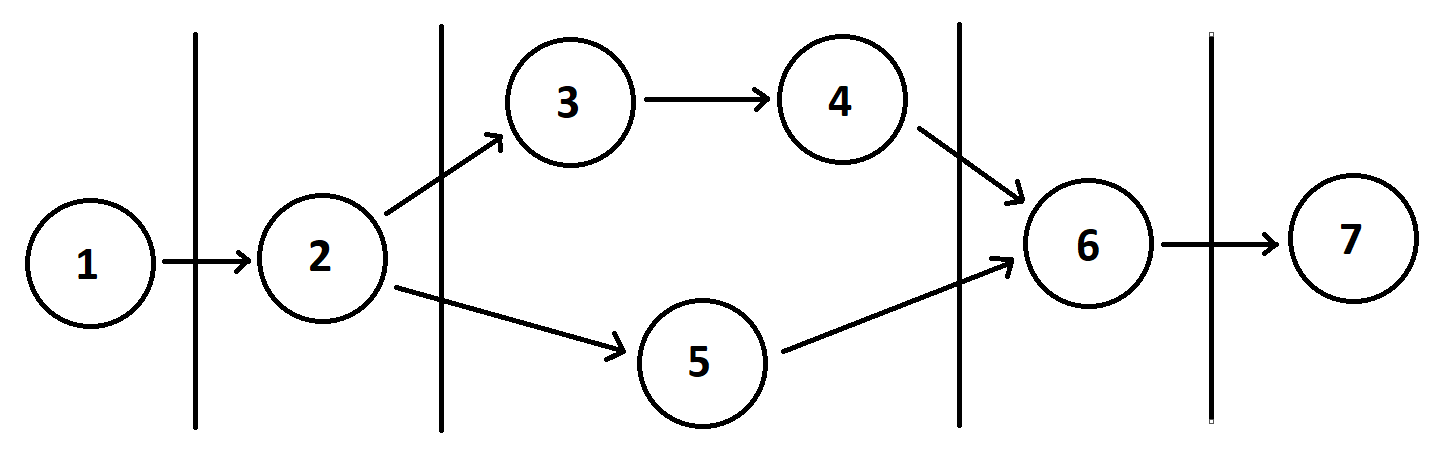
\includegraphics[width=0.4\linewidth]{Img/butcher/basic_graph.png}
    \caption{A graph. The vertical lines represent the different possible ways of partitioning the graph}
    \end{figure}
    
    \framebreak
    
    After this graph is constructed, extra nodes are added based on the number of devices: every node in the new graph should represent a specific collection of nodes in the original graph and a specific device. In this way, during the execution of the K shortest path algorithm, a path in the new graph will represent different partition elements of the network and the devices onto which they should be executed.
    
    \framebreak
    
        \begin{figure}[h]
        \centering
    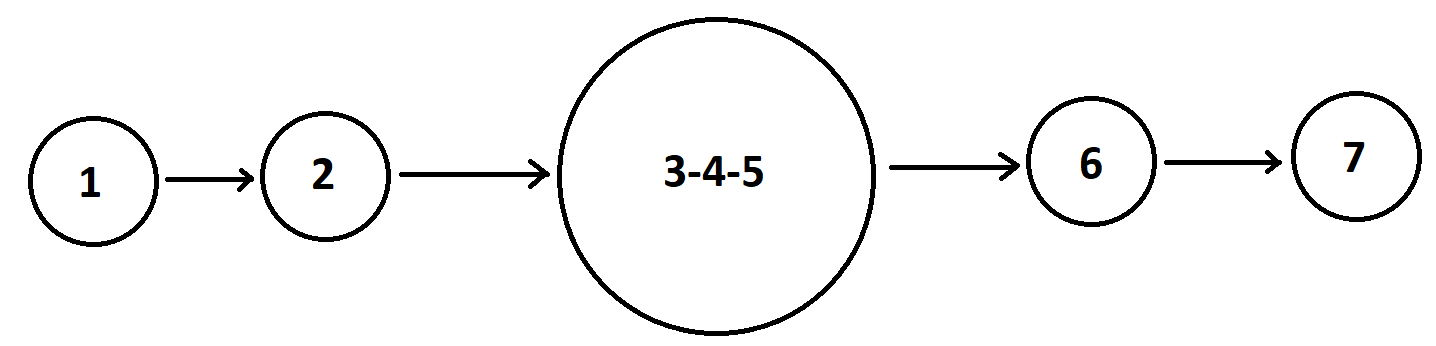
\includegraphics[width=0.4\linewidth]{Img/butcher/linearized_graph.png}
    \caption{First step in block graph construction}
    \end{figure}
    
    \begin{multicols}{2}
        \begin{figure}[h]
        \centering
    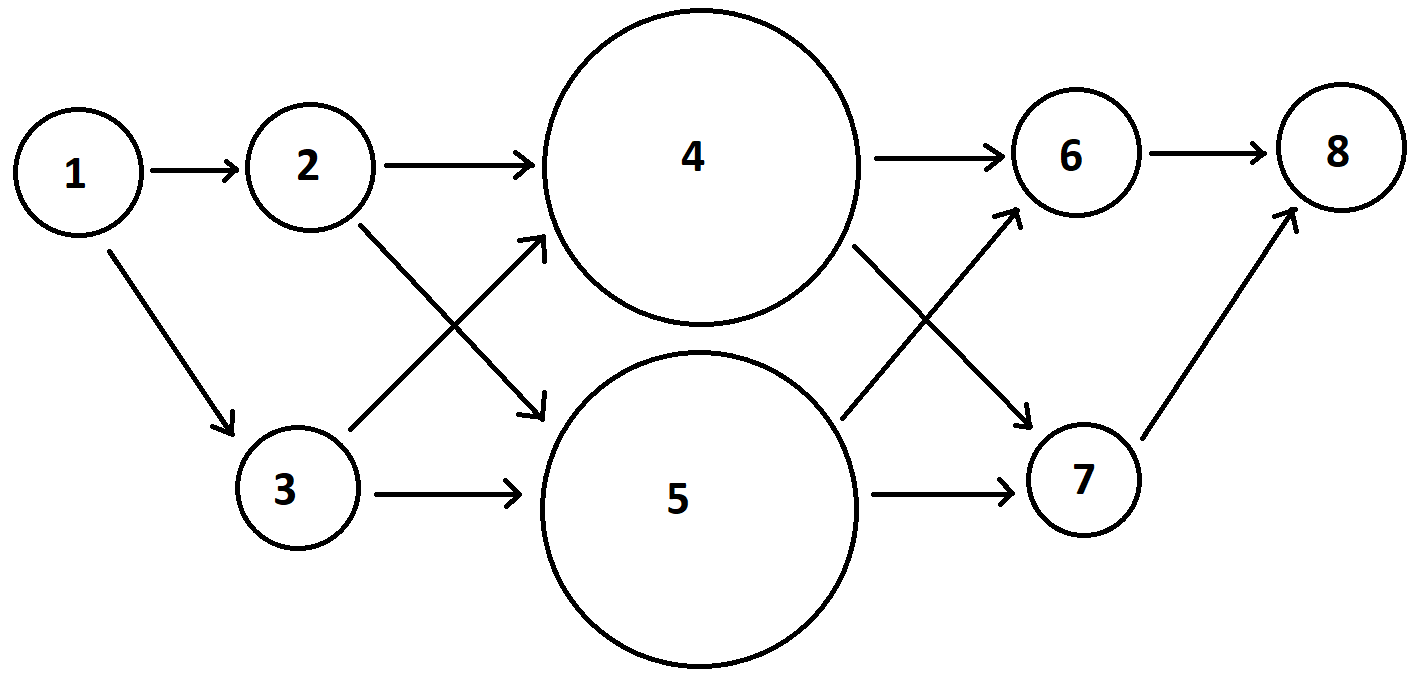
\includegraphics[width=0.75\linewidth]{Img/butcher/block_graph.png}
    \caption{The block graph}
    \end{figure}
    
        \begin{figure}[h]
        \centering
    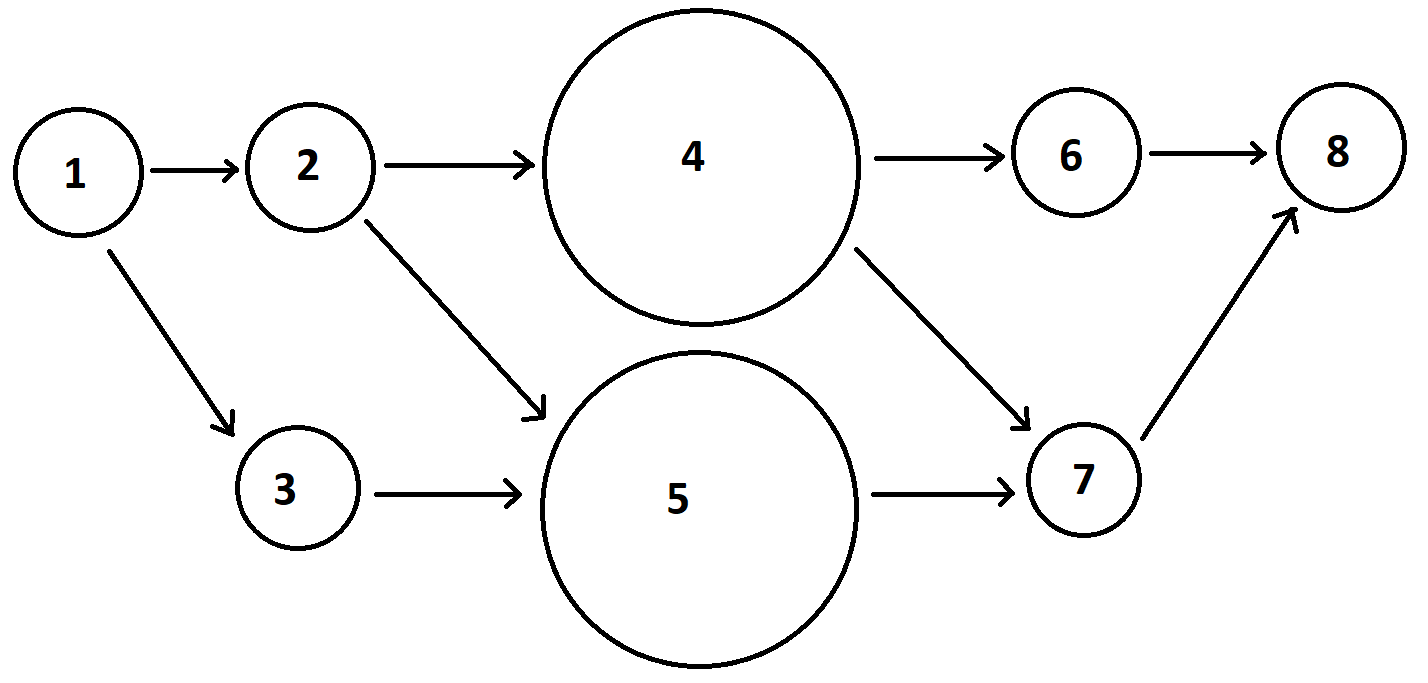
\includegraphics[width=0.75\linewidth]{Img/butcher/block_graph_no_backward_connections.png}
    \caption{The block graph (no backward connections)}
    \end{figure}
    \end{multicols}
    
    
    
\end{frame}

\begin{frame}{Memory constraint}
    \begin{block}{Basic idea}
    Every device has a maximum allowed memory capacity allocated for the execution of the NN. This means that, in theory, a partition of a NN may not be executable on a specific device. For this reason, based on the specified memory\_constraint\_type, some nodes and links in the block graph can be "safely" removed, since they are associated to unfeasible partitions.
    \end{block}
    
    If a node in the block graph corresponds to a single node in the original graph, we just measure the memory required by the input and output tensors. 
    
    If the node corresponds to multiple node in the original graph, we estimate the maximum memory required overall by this "block". 
    
    This estimate is done by computing the maximum input and output tensor dimensions and multiplying their sum by the number of tensors that, in the worst case, must be stored in memory.
\end{frame}

\begin{frame}{Import weights}
    The weights can be imported into the MWGraph through .csv files. There are three available import options:
    \begin{itemize}
        \item aMLLibrary: the .csv file is in the same format as the output file of the testing phase of the python aMLLibrary library. Note that, with this mode, only the weights associated to the convulutional layers are imported. 
        \item operation\_time: the .csv file is structured in a simple way: OperationTypeName,Weight. In this case, the program will read the operation reported in the .csv file and it will loop thorugh the nodes of the graph until the associated node is found. It will then add the related weight to the specified device
        \item multi\_operation\_time: the .csv file is structured in a simple way: OperationTypeName,Weight0,Weight1,... . In this case, the program will read the operation reported in the .csv file and it will loop through the nodes of the graph until the associated node is found. It will then add the related weights to all the devices
    \end{itemize}
\end{frame}

\begin{frame}{Transmission function}
    Since the objective of the program is to compute the optimal partitions for a given NN to be executed on different devices, we have to take into account that sending data from a device to another has a cost. 
    
    This cost is related to the memory space of the tensor to be sent. Moreover, this depends on the type of connection between the devices. 
    
    To simplify this process, we consider a transmission function that, based on the bandwidth parameters and the dimension of the tensor to be transmitted, will produce the related weight.
\end{frame}

\begin{frame}[allowframebreaks]{Weight generation}

    By "construction", the weight of a link represents the time required to transmit the tensor to another device (if needed) and the time required to execute the "input" node on the device specified by the "output" node.
    
    In the block graph, the weight of a link between two nodes is computed in the following way:
    \begin{itemize}
        \item If both nodes are associated to a single node in the original graph, then the resulting weight is given by the transmission cost and the weight between the corresponding nodes in the original graph on the device of the second node
        
    \begin{multicols}{2}
        \begin{figure}[h]
        \centering
    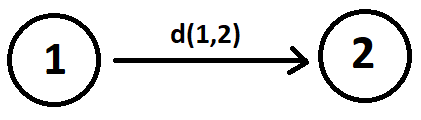
\includegraphics[width=0.5\linewidth]{Img/butcher/simple_edge.PNG}
    \caption{Edge in the original graph}
    \end{figure}
    
        \begin{figure}[h]
        \centering
    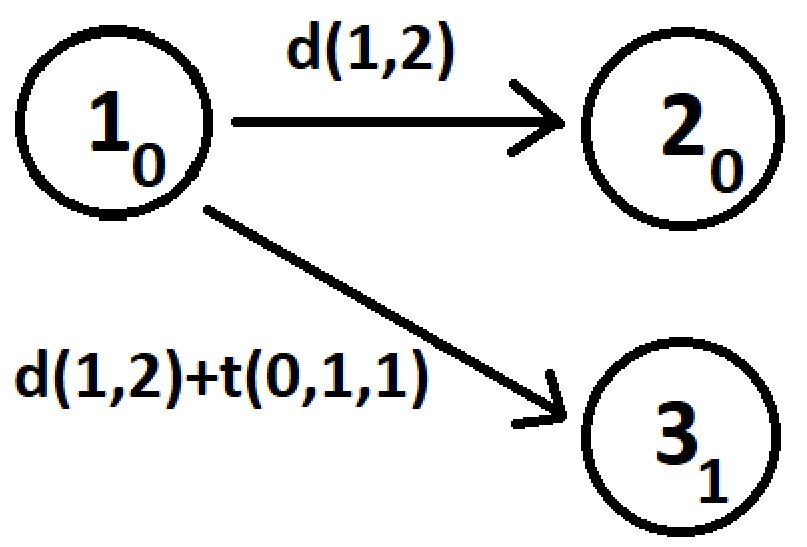
\includegraphics[width=0.4\linewidth]{Img/butcher/block_edge.PNG}
    \caption{Related edges in the block graph}
    \end{figure}
    \end{multicols}
        
        \framebreak
        
        \item If the first node corresponds to a single node in the original graph while the second one to multiple nodes, then the transmission cost for the output tensor of the first node is summed with the different weights between the first node correspondent on the original graph with the "children" nodes in the original graph, plus all the costs between the nodes contained in the second node of the new graph
        
        
    \begin{multicols}{2}
        \begin{figure}[h]
        \centering
    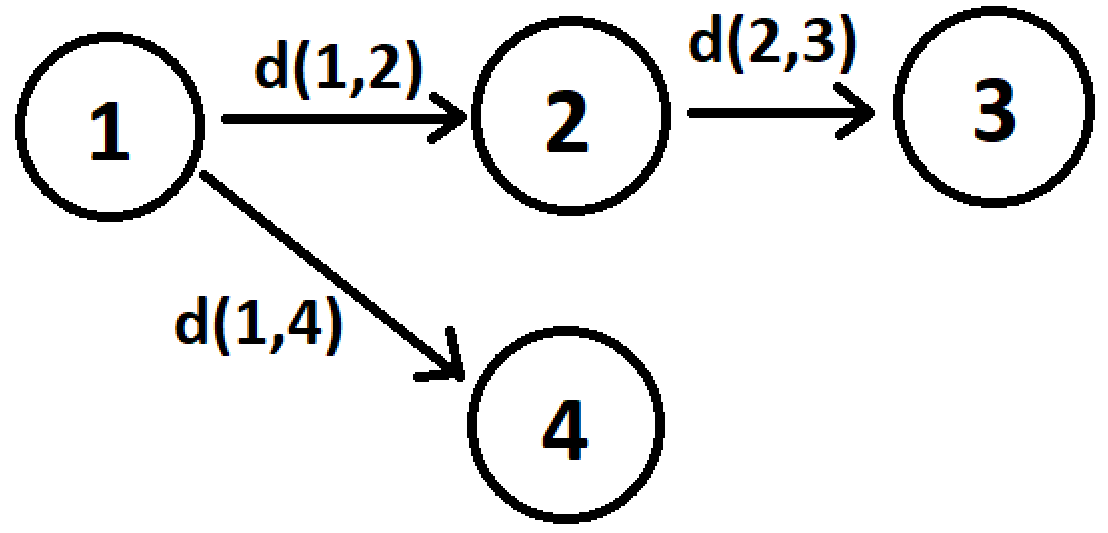
\includegraphics[width=0.5\linewidth]{Img/butcher/2_1_simple_edge.PNG}
    \caption{Edge in the original graph}
    \end{figure}
    
        \begin{figure}[h]
        \centering
    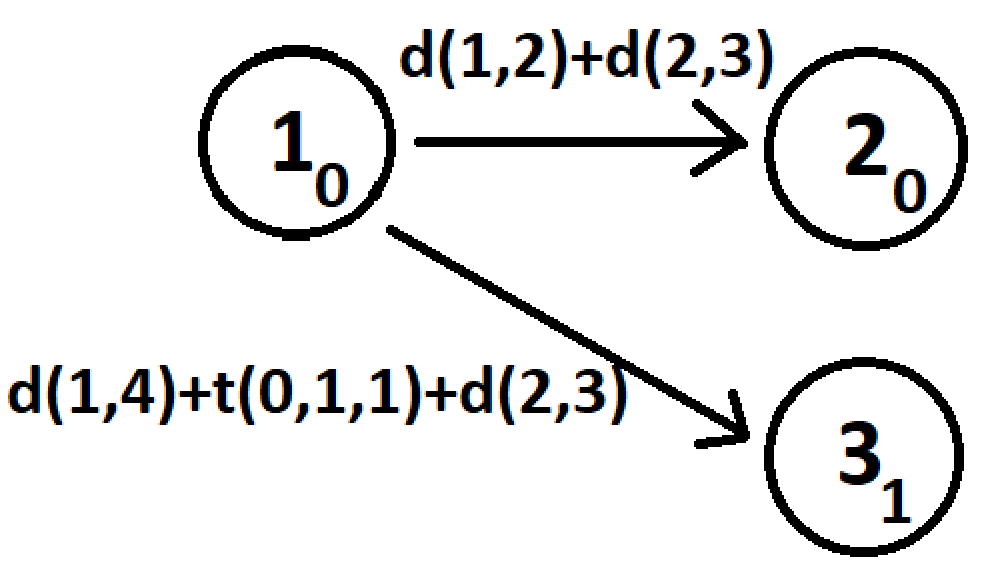
\includegraphics[width=0.7\linewidth]{Img/butcher/2_1_block_edge.PNG}
    \caption{Related edges in the block graph}
    \end{figure}
    \end{multicols}
        
        \framebreak
        
        \item If the first node corresponds to multiple nodes in the original graph while the second one to a single node, then the transmission cost is considered for all the tensors that must be transmitted to the second node plus the costs associated to the links between the input nodes (on the original graph) of the second node in the new graph
        
        
    \begin{multicols}{2}
        \begin{figure}[h]
        \centering
    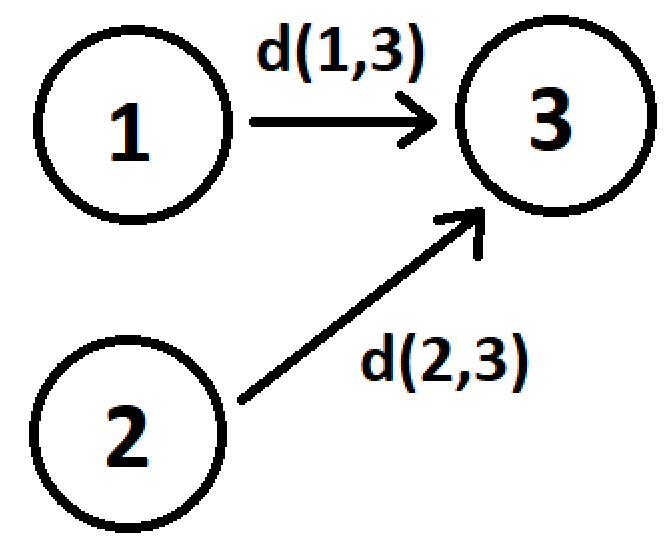
\includegraphics[width=0.4\linewidth]{Img/butcher/1_2_simple_edge.PNG}
    \caption{Edge in the original graph}
    \end{figure}
    
        \begin{figure}[h]
        \centering
    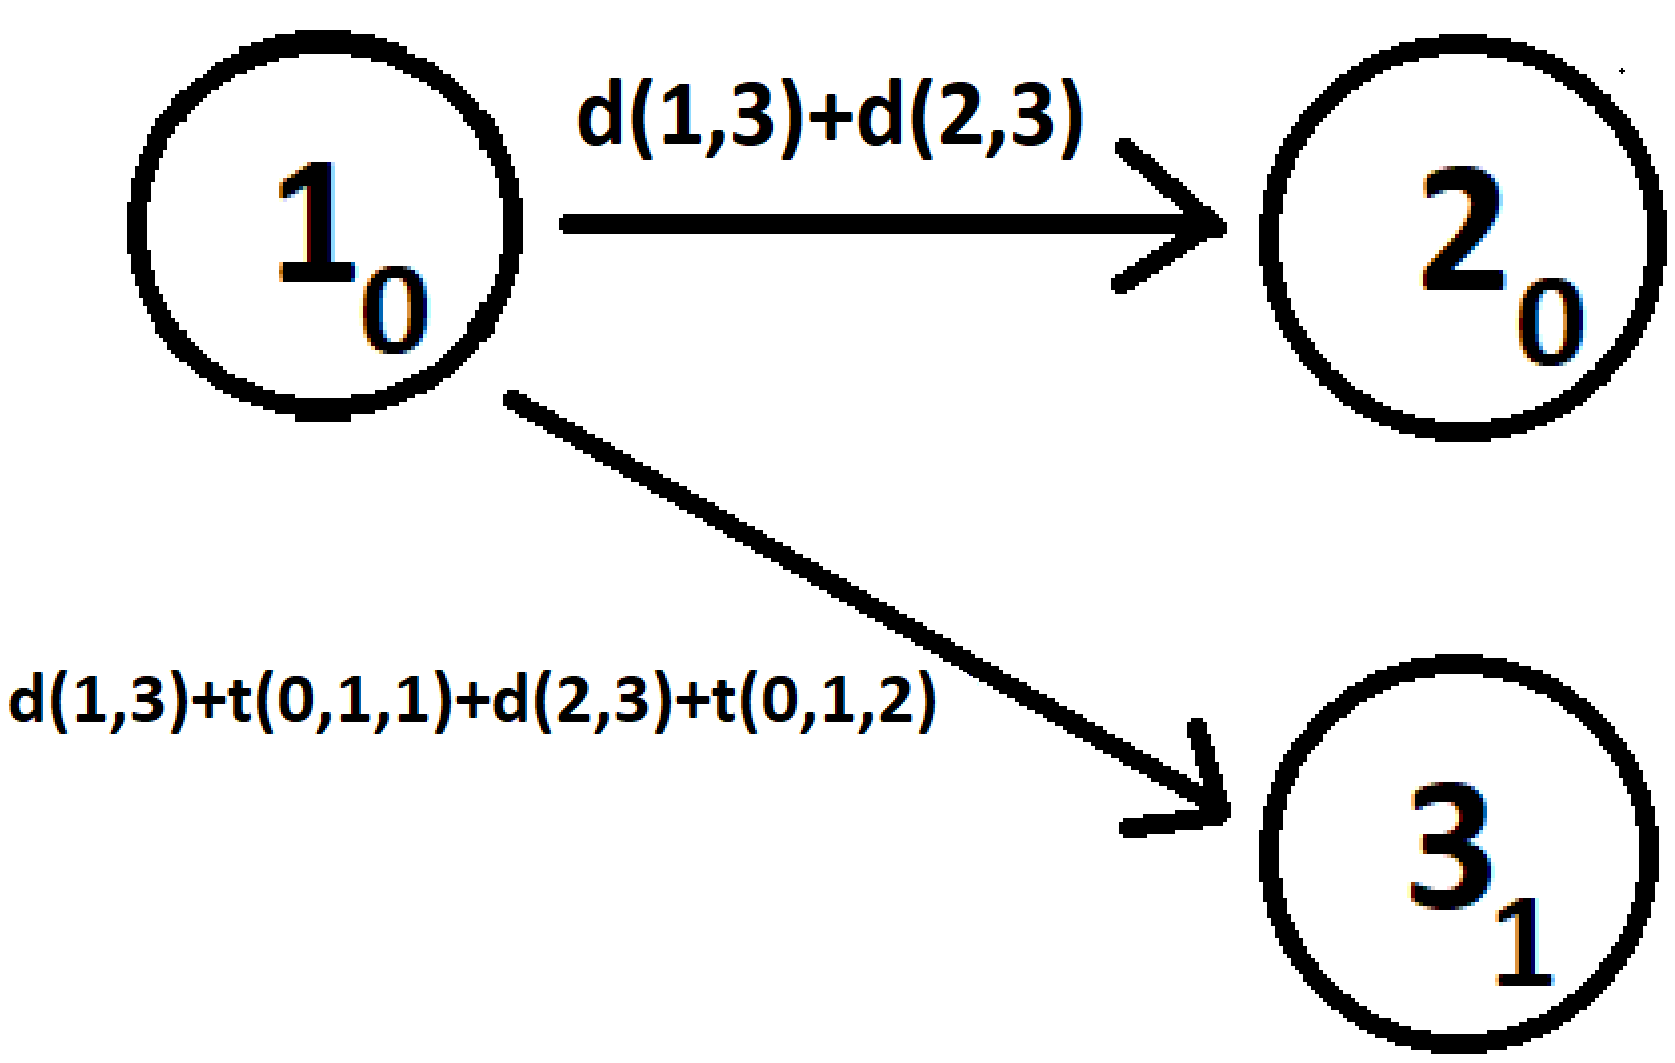
\includegraphics[width=0.6\linewidth]{Img/butcher/1_2_block_edge.PNG}
    \caption{Related edges in the block graph}
    \end{figure}
    \end{multicols}
    
    \end{itemize}
    
\end{frame}
\section{K Shortest Path}

\begin{frame}[plain]{}
    \sectionpage
\end{frame}
\section{Model reconstruction and export}

\begin{frame}[plain]{}
    \sectionpage
\end{frame}

\begin{frame}{Model reconstruction and export}
    Once the K shortest path method is applied to the "block" graph, the following steps must be performed:
\begin{enumerate}
    \item Construction of the associated path in the original graph, taking into account the device onto which every node must be runned. 
    \item Generate the different onnx::ModelProto associated to the different sub-graphs of the original graph. Every onnx::ModelProto is associated to a specific device
    \item Finally, the different onnx::ModelProto are exported in the .onnx file in the specified directory
\end{enumerate}

\end{frame}
\section{Experiments}

\begin{frame}[plain]{}
    \sectionpage
\end{frame}

\begin{frame}{Some numerical results}

\begin{table}[]
\begin{tabular}{|c|c|c|c|}
\hline
\textbf{Name}      & \textbf{backward\_connections} & \textbf{num\_devices} & \textbf{K}        \\ \hline
RFB\_640  & false                          & 3                     & 1000              \\ \hline
MobileNet & false                          & 2                     & 1000 (actual 100) \\ \hline
MobileNet & false                          & 3                     & 1000              \\ \hline
\end{tabular}
\end{table}

\begin{table}[]
\begin{tabular}{|c|c|c|c|c|}
\hline
\textbf{Name} & \textbf{Network import {[}ns{]}} & \textbf{Weight import {[}ns{]}} & \textbf{Butchering {[}ns{]}} & \textbf{Export {[}ns{]}} \\ \hline
RFB\_640 & 11834,8 & 445,198 & 60270,1 & 2,68E+07 \\ \hline
MobileNet          & 17611,8 & 639,706 & 4332,4  & 981519   \\ \hline
MobileNet          & 18059,8 & 760     & 41282,7 & 1,47E+08 \\ \hline
\end{tabular}
\end{table}

\end{frame}


\end{document}